\chapter{Development Timeline}
Below is our development timeline in a Gantt chart format. A Gantt chart lays out each member's tasks in an easy to view, timeline format. Develop Project Specification is when Sathya figures out the product's requirements. Setting up the coding environment is when Kevin researches how we can start the coding part and gets it ready. Wil analyzes the current solutions and how we can improve upon them at this time. Usability is keeping the app usable and adding features to make it more usable. Prototypes will be used to show our idea to our adviser and potential customers. The design document contains our ideas and explains them to our adviser and others. Testing occurs throughout the coding process. Wil will find people with ASD to test our product and give us ways to improve Emojent. We will all be coding and documenting but Kevin is in charge of the documentation. This means he will check it thoroughly and make fixes. Finally, we will prepare for our presentation and present Emojent in late May or early June. 
\begin{sidewaysfigure}
    \centering
    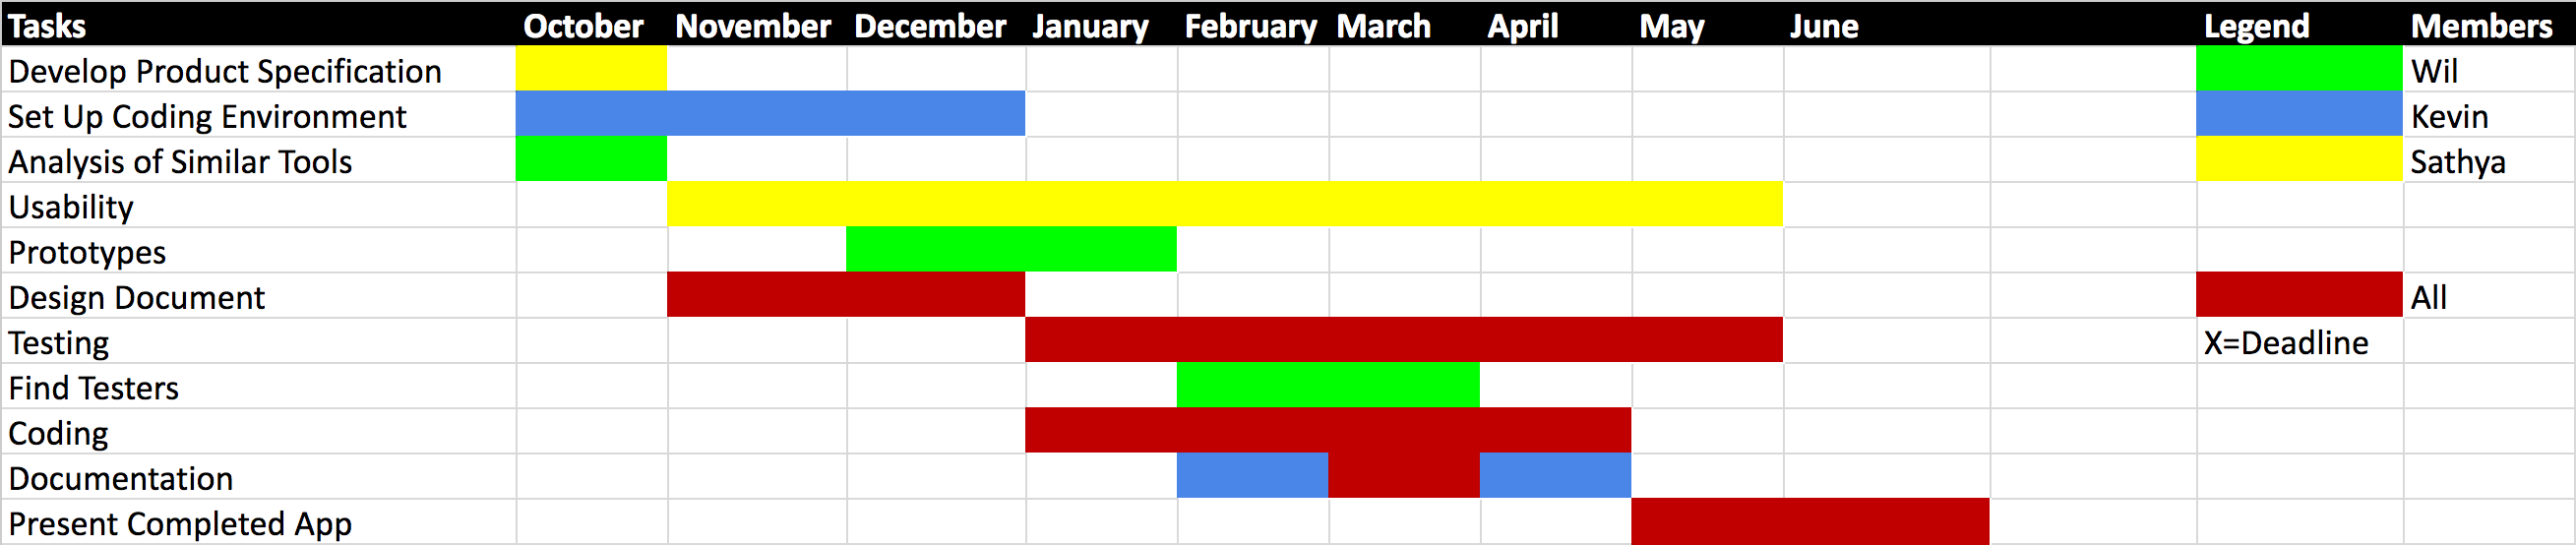
\includegraphics[scale=.5]{ganttChart.png}  
    \caption{\label{fig:Development Timeline}Development Timeline.} 
\end{sidewaysfigure}